\documentclass[tikz,border=8pt]{standalone}
\usepackage{xcolor}
\usetikzlibrary{arrows.meta,positioning,shapes.geometric}
\tikzset{
  process/.style={
    draw,
    rounded corners=4pt,
    minimum width=4.2cm,
    minimum height=0.95cm,
    text width=4.0cm,
    align=center,
    font=\small,
    fill=blue!8
  },
  io/.style={
    draw,
    rounded corners=4pt,
    minimum width=4.2cm,
    minimum height=0.95cm,
    text width=4.0cm,
    align=center,
    font=\small,
    fill=green!8
  },
  decision/.style={
    draw,
    diamond,
    aspect=2.0,
    minimum width=2.8cm,
    minimum height=1.1cm,
    align=center,
    font=\small,
    fill=orange!10
  },
  note/.style={
    draw,
    dashed,
    rounded corners=4pt,
    text width=4.4cm,
    align=left,
    font=\scriptsize,
    fill=gray!6
  },
  flow/.style={->, >=Latex, thick, draw=gray!70}
}
\begin{document}
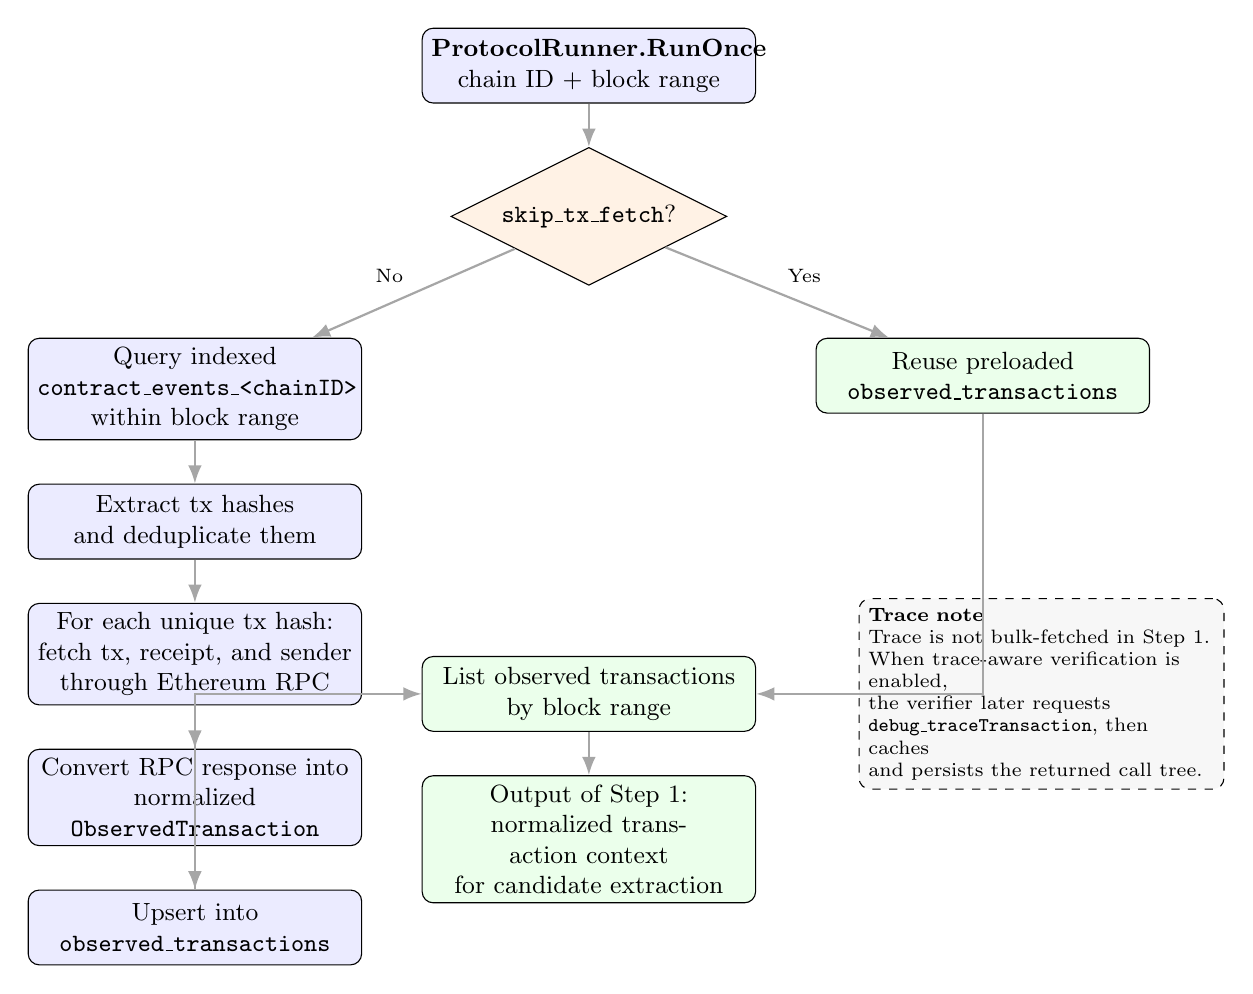
\begin{tikzpicture}[node distance=0.55cm]
  \node[process] (start) {\textbf{ProtocolRunner.RunOnce}\\chain ID + block range};
  \node[decision, below=of start] (skip) {\texttt{skip\_tx\_fetch}?};

  \node[process, below left=1.1cm and 2.0cm of skip] (query) {Query indexed\\\texttt{contract\_events\_<chainID>}\\within block range};
  \node[process, below=of query] (dedup) {Extract tx hashes\\and deduplicate them};
  \node[process, below=of dedup] (rpc) {For each unique tx hash:\\fetch tx, receipt, and sender\\through Ethereum RPC};
  \node[process, below=of rpc] (normalize) {Convert RPC response into\\normalized \texttt{ObservedTransaction}};
  \node[process, below=of normalize] (upsert) {Upsert into\\\texttt{observed\_transactions}};

  \node[io, below right=1.1cm and 2.0cm of skip] (reuse) {Reuse preloaded\\\texttt{observed\_transactions}};
  \node[io, below=4.7cm of skip] (list) {List observed transactions\\by block range};
  \node[io, below=of list] (output) {Output of Step 1:\\normalized transaction context\\for candidate extraction};

  \node[note, right=1.3cm of list] (trace) {\textbf{Trace note}\\Trace is not bulk-fetched in Step 1.\\When trace-aware verification is enabled,\\the verifier later requests\\\texttt{debug\_traceTransaction}, then caches\\and persists the returned call tree.};

  \draw[flow] (start) -- (skip);
  \draw[flow] (skip) -- node[midway, above left, font=\scriptsize]{No} (query);
  \draw[flow] (query) -- (dedup);
  \draw[flow] (dedup) -- (rpc);
  \draw[flow] (rpc) -- (normalize);
  \draw[flow] (normalize) -- (upsert);
  \draw[flow] (skip) -- node[midway, above right, font=\scriptsize]{Yes} (reuse);
  \draw[flow] (upsert) |- (list);
  \draw[flow] (reuse) |- (list);
  \draw[flow] (list) -- (output);
\end{tikzpicture}
\end{document}
